%%%%%%%%%%%%%%%%%%%%%%%%%%%%%%%%%%%%%%%%%%%%%%%%%%%%%%%%%%%%%%%%%%%%%%%%%%%%%%%%
%2345678901234567890123456789012345678901234567890123456789012345678901234567890
%        1         2         3         4         5         6         7         8

\documentclass[conference]{IEEEtran}  % Comment this line out
                                                          % if you need a4paper
%\documentclass[a4paper, 10pt, conference]{ieeeconf}      % Use this line for a4
                                                          % paper

\IEEEoverridecommandlockouts                              % This command is only
                                                          % needed if you want to
                                                          % use the \thanks command
%\overrideIEEEmargins
% See the \addtolength command later in the file to balance the column lengths
% on the last page of the document
\usepackage{graphics}
\usepackage{hyperref}
\hypersetup{
    colorlinks=true,
    linkcolor=blue,
    filecolor=magenta,      
    urlcolor=blue,
    pdftitle={Overleaf Example},
    pdfpagemode=FullScreen,
    }
\usepackage{amsmath}
\usepackage[export]{adjustbox}% http://ctan.org/pkg/adjustbox
\usepackage{graphicx}
% The following packages can be found on http:\\www.ctan.org
%\usepackage{graphics} % for pdf, bitmapped graphics files
%\usepackage{epsfig} % for postscript graphics files
%\usepackage{mathptmx} % assumes new font selection scheme installed
%\usepackage{times} % assumes new font selection scheme installed
%\usepackage{amsmath} % assumes amsmath package installed
%\usepackage{amssymb}  % assumes amsmath package installed

\title{\LARGE \bf
Soft Binarized Neural Network for Inference using \\ RRAM Crossbars with Minimal Quantization Errors
}

%\author{ \parbox{3 in}{\centering Huibert Kwakernaak*
%         \thanks{*Use the $\backslash$thanks command to put information here}\\
%         Faculty of Electrical Engineering, Mathematics and Computer Science\\
%         University of Twente\\
%         7500 AE Enschede, The Netherlands\\
%         {\tt\small h.kwakernaak@autsubmit.com}}
%         \hspace*{ 0.5 in}
%         \parbox{3 in}{ \centering Pradeep Misra**
%         \thanks{**The footnote marks may be inserted manually}\\
%        Department of Electrical Engineering \\
%         Wright State University\\
%         Dayton, OH 45435, USA\\
%         {\tt\small pmisra@cs.wright.edu}}
%}

\author{Rishi Nandha V (EE21B111), Satvik Malapaka (EE21B080)\\
Department of Electrical Engineering, IIT Madras\\
% <-this % stops a space
% <-this % stops a space
%
}



\begin{document}



\maketitle
\thispagestyle{empty}
\pagestyle{empty}


%%%%%%%%%%%%%%%%%%%%%%%%%%%%%%%%%%%%%%%%%%%%%%%%%%%%%%%%%%%%%%%%%%%%%%%%%%%%%%%%
\begin{abstract}

The increasing demand for energy-efficient hardware to implement neural networks has become crucial, driven by the rising interest in Generative AI algorithms. RRAM crossbars have emerged as a promising solution for such implementations due to their high parallelism and energy efficiency. In this work, we propose a new technique, Soft Binarization, which approximates binary behavior of weights during the ex-situ training to align neural network models with RRAM crossbar characteristics.  By incorporating this approach during training, quantization-induced errors are minimized, and hardware-software alignment is improved. Notably, we demonstrate that the accuracy drop due to quantization-induced errors can be reduced to as low as \textbf{2\%}.

\end{abstract}


%%%%%%%%%%%%%%%%%%%%%%%%%%%%%%%%%%%%%%%%%%%%%%%%%%%%%%%%%%%%%%%%%%%%%%%%%%%%%%%%
\section{Introduction}
The increasing computational demands of neural networks have led to significant interest in in-memory computing and neuromorphic computing paradigms. In-memory computing minimizes energy overhead by performing computations directly within memory, thereby eliminating the need for frequent data transfers between memory and processing units. A notable approach is to translate matrix multiplications—central to neural network operations—into the interaction of input voltages with stored conductance values, producing current outputs.

This functionality can be realized using \textbf{RRAM-based crossbar arrays}, where electrodes intersect at memory cells that simultaneously store synaptic weights (as conductance) and perform computation. \textbf{Resistive Random-Access Memory (RRAM)}, a non-volatile device exhibiting electric hysteresis, can reliably be programmed into \textbf{ON} or \textbf{OFF} states. This makes crossbars with RRAMs as the memory cells an attractive solution for implementing energy-efficient neural network accelerators.

Previous work has demonstrated the feasibility of implementing neural networks using RRAM crossbar arrays. Li \textit{et al.}~\cite{b1} successfully employed a crossbar-based approach to implement a multilayer perceptron. While their primary work was introducing a feedback-based programming method to support continuous weights rather than binary (ON/OFF), they've also demonstrated that converting continuous weights to binary weights, resulted in a significant accuracy drop of about \textbf{15.6\%}. We refer to such a drop in accuracy due to binarization of weights as the \textbf{quantization error in inference}.

In this work, we proceed with a binary programming approach and focus on minimizing quantization errors by accounting for the binary nature of weights during ex-situ training. Although this method introduces a slight accuracy reduction in software inference, it ensures a more reliable performance replication in hardware inference. To achieve this, we propose a technique termed "Soft Binarization". Additionally, we also use activation functions that closely fit the characteristic of the real circuit element that will be used in the hardware implementation. With this methodology, we demonstrate that the accuracy drop can be reduced to as low as \textbf{2\%} for the same dataset used by Li \textit{et al.}\cite{b1}. The training set is illustrated in Fig.\ref{fig:1}.


\begin{figure}[h]
    \centering
    \includegraphics[width=1\linewidth]{Training_Set.png}
    \caption{Training Images from the Dataset}
    \label{fig:1}
\end{figure}
\vspace*{-3mm}
\section{Soft Binarized Neural Network} 

To model the behavior of the RRAM cells, we approximate that, under the same writing voltage, the conductance in all RRAM cells identically becomes the same, thereby neglecting variations. We denote this conductance in the ON state as \( G_{\text{ON}} \). In reality, the conductance also exhibits non-linearity with respect to the reading voltage; however, to a small-signal extent, we neglect these deviations. Similarly, the conductance in the OFF state is denoted as \( G_{\text{OFF}} \). 

The table below summarizes the RRAM parameters used in the \textbf{Stanford compact model}~\cite{b2}, including the writing and reading voltages, observed \( G_{\text{ON}} \) and \( G_{\text{OFF}} \), and the validity range of the small-signal approximation.

\vspace*{-1mm}
\begin{table}[h]
    \centering
    \renewcommand{\arraystretch}{1.5} % Add padding (1.5 times line height)
    \setlength{\tabcolsep}{1mm}       % Add 1mm horizontal padding
    \begin{tabular}{|c|c|c|}
    \hline
        Gap Coefficient $\mathbf{g_0}$ & Voltage Coefficient $\mathbf{V_0}$ & Prefactor $\mathbf{I_0}$ \\\hline
        0.94 nm & 0.21 V & 19.5 $\mu$A \\\hline
    \end{tabular}\\
    \vspace*{2mm}
    \renewcommand{\arraystretch}{1.5} % Ensure padding for second table
    \begin{tabular}{|c|c|c|c|}
    \hline
        Escape Velocity $v_0$ & $\beta$~\cite{b2} & $\gamma_0$~\cite{b2} & $\alpha$~\cite{b2} \\\hline
        $1 \times 10^7$ & 9.0 & 30 & 0.5 \\\hline
    \end{tabular}\\
    \vspace*{2mm}
    \renewcommand{\arraystretch}{1.5} % Ensure padding for third table
    \begin{tabular}{|c|c|c|c|c|}
    \hline
        $V_{\text{WRITE}}$ & $V_{\text{READ}}$ & $G_{\text{ON}}$ & $G_{\text{OFF}}$ & Small-Signal \\\hline
        1.5 V & $\pm$0.1 V & $7.7 \times 10^{-5}$ & $2.88 \times 10^{-6}$ & $\pm$ 0.15 V \\\hline
    \end{tabular}
\end{table}

To minimize the accuracy drop caused by quantization errors, we address the fundamental reason for this disparity—\textbf{the forward pass in conventional neural networks employs continuous weights}, whereas RRAM-based hardware is restricted to discrete values \( G_{\text{ON}} \) or \( G_{\text{OFF}} \). A straightforward approach would be to binarize the weights in software; however, this introduces a non-differentiable computation graph, causing the back-propagation process to fail. 

To resolve this issue, we apply a sigmoid or tanh activation to the weights, which approximates a binary step function while retaining differentiability. This operation is performed prior to matrix multiplication during forward propagation, with the range of the weights constrained between \( G_{\text{ON}} \) and \( G_{\text{OFF}} \). Additionally, we introduce a prefactor \(\zeta\), referred to as the \textbf{sharpness}, as a hyperparameter to prevent gradients during back-propagation from vanishing.

\vspace*{-3mm}
\begin{equation}
\textbf{soft\_bin}\left(x\right) = \left(G_{\text{ON}} - G_{\text{OFF}}\right) \cdot \textbf{sigmoid}\left(\zeta \cdot x\right) + G_{\text{OFF}}
\end{equation}


Thus, the forward propagation equation is defined as follows, where the superscript corresponds to the layer index, the subscript corresponds to the neuron's index within that layer, \( g \) denotes the activation function of the layer, and \( a \) represents the activation of the neuron:

\vspace*{-2mm}
\begin{equation}
a^{[l+1]}_{i} = g^{[l+1]} \left(\sum_k \textbf{soft\_bin}\left(w_{ik}\right) \cdot a^{[l]}_k \right)
\end{equation}

For our dataset, we implement a neural network with three layers, containing 16, 8, and 4 neurons, respectively. The computation graph of the network is illustrated in Fig.~\ref{fig:2}. Soft\_Bin() is the function discussed above. InvAmp() is the activation function discussed in the next section

\begin{figure}[h]
    \centering
    \includegraphics[width=1\linewidth]{SBNN.png}
    \caption{Computation Graph}
    \label{fig:2}
\end{figure}
\vspace*{-3mm}
\section{Inverting Amplifier Activation}

The neural network needs an activation function between the two layers to effectively learn non-linear trends in the training data. The current mode output of the RRAM crossbar also needs to be converted into a voltage mode signal for the next crossbar's input. To serve both of these purposes, we design an inverting amplifier using an inverter in negative feedback with a resistor. 

As a result, in the forward pass of the network shown in figure \ref{fig:2}, InvAmp() is defined as the following:

\begin{equation}
    \textbf{InvAmp}(x) = V_{\text{RAIL}} \cdot \tanh\left(\frac{x \cdot R_{\text{fb}}}{V_{\text{RAIL}}}\right)
\end{equation}

Figure \ref{fig:3} shows one such Inverting Amplifier and it's input current vs output voltage characteristic showing a tanh behavior.

\begin{figure}[h]
    \centering
    \includegraphics[width=1\linewidth]{INVAMP.png}
    \caption{\textbf{a.} InvAmp() Charecteristic \textbf{b.} Inverter in Negative Feedback}
    \label{fig:3}
\end{figure}

Note that the choice of $R_{\text{fb}}$ is critical to how the network behaves because it gives the gain of this amplifier stage. A resistance that is too large will result in input voltages to the second crossbar stage to exceed the small-signal limits. A resistance that is too small will not produce legible results.

\section{Training \& Implementation}
For training the neural network, a learning rate warm-up and fine-tuning schedule were applied. The network, implemented as a custom PyTorch class with circuit parameters as hyperparameters, utilized Xavier Uniform initialization with a small spread. Voltage values after the first inverting amplifier stage were monitored during training to optimize \( R_{\text{fb}} \). Data augmentation included Dropout and noise injection. Input 1s and 0s were mapped to $+V_{\text{READ}}$ and $-V_{\text{READ}}$. Figure~\ref{fig:4} presents the accuracy and loss curves over epochs.


\begin{figure}[h]
    \centering
    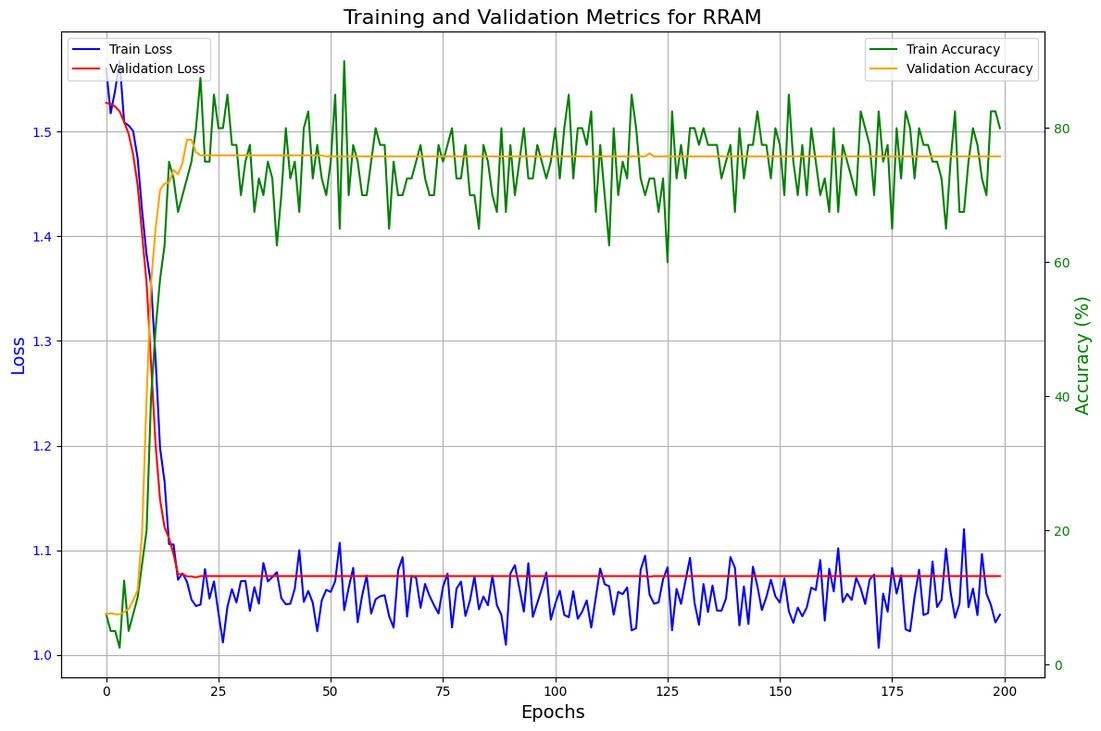
\includegraphics[width=1\linewidth]{Training_Plot.png}
    \caption{Training Plot}
    \label{fig:4}
\end{figure}

The following table summarizes parameters used:

\begin{table}[h]
    \centering
    \renewcommand{\arraystretch}{1.3} % Increase row padding
    \setlength{\tabcolsep}{4pt} % Increase column padding
    \begin{tabular}{|c|c|c|c|c|} \hline
         $\zeta$ & $V_{\text{RAIL}}$ & $R_{\text{fb}}$ & $V_0$ & $V_1$\\ \hline
         500 & 1.2 V & 2 k$\Omega$ & 0.1 V & -0.1 V\\ \hline
    \end{tabular}
\end{table}

For programming these, 100$\mu$s pulses and a V/3 Scheme were used. We have to isolate the crossbars during programming and then connect them through the Inverting Amplifiers for inference, hence Analog MUXes were made and used. Figure \ref{fig:5} shows the internal construction

\begin{figure}[h]
    \centering
    \includegraphics[width=0.35\linewidth]{A_MUX.png}
    \caption{Analog MUX using Transition Gates}
    \label{fig:5}
\end{figure}

Figure \ref{fig:6} shows a reduced equivalent that demonstrates how the switching between programming and inference is implemented and shows the complete path from the input till the output through the RRAMs, MUXes and Inverting Amplifiers

\begin{figure}[h]
    \centering
    \includegraphics[width=1\linewidth]{analog_mux_prop_path.png}
    \caption{Setup for switching between programming and inference}
    \label{fig:6}
\end{figure}

Our notebook used for training the Neural Network including the Custom PyTorch class can be found \href{https://github.com/RishiNandha/CMOS-Binary-Neural-Network/blob/main/BNN.ipynb}{here} and our final model file can be found \href{https://github.com/RishiNandha/CMOS-Binary-Neural-Network/blob/main/RRAM_model_78%25.pth}{here}

\section{Results}

Figure \ref{fig:7} shows the complete circuit for the 3 - layer Neural Network made of 2 RRAM Crossbars, Inverting Amplifiers and Switching MUXes

\begin{figure}[h]
    \centering
    \includegraphics[width=1\linewidth]{full_circuit.png}
    \caption{Full Circuit}
    \label{fig:7}
\end{figure}

Figure \ref{fig:8} shows the output voltages for inference of 16 images as a short demonstration of the appropriate working of the setup. (RED = A\_pred, NAVY BLUE = X\_pred, PINK = V\_pred, LIGHT BLUE = T\_pred)

\begin{figure}[h]
    \centering
    \includegraphics[width=1\linewidth]{accuracy.png}
    \caption{Demonstration of Inference on 16 Images}
    \label{fig:8}
\end{figure}

Further, we compare software training accuracy, software testing accuracy and simulation testing accuracy on 160 testing images in the table presented below

\renewcommand{\arraystretch}{1.3} % Adjust row height
\setlength{\tabcolsep}{6pt}       % Adjust column spacing

\begin{table}[h]
    \centering
    \begin{tabular}{|c|c|}\hline
        Software Training Accuracy &  \textbf{87.5\%} \\ \hline
        Software Testing Accuracy on 640 Images & \textbf{78.3\%} \\ \hline
        Software Testing Accuracy on 160 Images & \textbf{80.6\%} \\ \hline
        Simulation Testing Accuracy on 160 Images & \textbf{78.8\%}\\ \hline
    \end{tabular}
\end{table}

The table below compares the Accuracy Drop due to Quantization Error in this work and that shown in \cite{b1} with binary weights ("Hardware-Unaware" as per that work's terminology).

\renewcommand{\arraystretch}{1.3} % Adjust row height
\setlength{\tabcolsep}{4pt}       % Adjust column spacing

\begin{table}[h]
    \centering
    \begin{tabular}{|c|c|c|c|}\hline
         ~ & Software Acc. & Crossbar Acc. & Drop due to Quantization\\ \hline
         Li \textit{et al.} \cite{b1} & \textbf{95\%} & \textbf{79.4\%}&\textbf{15.6\%}\\ \hline
         This work & \textbf{80.6\%}&\textbf{78.8\%} & \textbf{1.8\%}\\ \hline
    \end{tabular}
\end{table}

Figure \ref{fig:9} shows the scatter plot of predictions. Our ADS Workspace can be found \href{https://github.com/RishiNandha/CMOS-Binary-Neural-Network/blob/main/78.5%25_Accuracy.7zads}{here}

\begin{figure}[h]
    \centering
    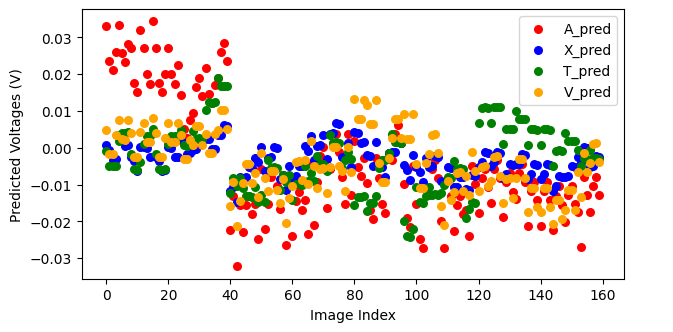
\includegraphics[width=0.85\linewidth]{Predictions_Scatter.png}
    \caption{Predictions Scatter Plot}
    \label{fig:9}
\end{figure}

\begin{thebibliography}{00}
\bibitem{b1} H. Li et al., “Analogue signal and image processing with large memristor crossbars,” Nature Communications, vol. 9, no. 1, p. 2385, 2018, doi: 10.1038/s41467-018-04482-4
\bibitem{b2} Z. Jiang et al., "A compact model for metaloxide resistive random access memory with experiment verification", IEEE Trans. Electron Devices, vol. 63, no. 5, pp. 1884-1892, May 2016
\end{thebibliography}

\end{document}


